\documentclass[12pt]{article}

% This first part of the file is called the PREAMBLE. It includes
% customizations and command definitions. The preamble is everything
% between \documentclass and \begin{document}.

\usepackage[margin=1in]{geometry}  % set the margins to 1in on all sides
\usepackage{graphicx}              % to include figures
\usepackage{amsmath}               % great math stuff
\usepackage{amsfonts}              % for blackboard bold, etc
\usepackage{amsthm}                % better theorem environments
\usepackage{amssymb} 
\usepackage{mathptmx}
\usepackage{graphicx}
\usepackage{listings}
\usepackage{xcolor}

% various theorems, numbered by section

\newtheorem{thm}{Theorem}[section]
\newtheorem{lem}[thm]{Lemma}
\newtheorem{prop}[thm]{Proposition}
\newtheorem{cor}[thm]{Corollary}
\newtheorem{conj}[thm]{Conjecture}
\newtheorem{mydef}[thm]{Definition}


\lstset{
	basicstyle          =   \sffamily,          
	keywordstyle        =   \bfseries,          
	commentstyle        =   \rmfamily\itshape,  
	stringstyle         =   \ttfamily,  
	flexiblecolumns,                
	numbers             =   left,   
	showspaces          =   false,  
	numberstyle         =   \fontsize{5}{skip},    
	showstringspaces    =   false,
	captionpos          =   t,      
	frame               =   lrtb,   
}

\lstdefinestyle{cpp}{
	language        =   cpp, 
	basicstyle      =   \fontsize{5}{skip},
	numberstyle     =   \fontsize{5}{skip},
	keywordstyle    =   \color{blue},
	keywordstyle    =   [2] \color{teal},
	stringstyle     =   \color{magenta},
	commentstyle    =   \color{red}\ttfamily,
	breaklines      =   true,   
	columns         =   fixed,  
	basewidth       =   0.5em,
}
\begin{document}


\title{ CSE 102 Spring 2021\\
	Advanced Homework Assignment 3}

\author{Jaden Liu \\ 
University of California at Santa Cruz\\
Santa Cruz, CA 95064 USA }

\maketitle


\section{AdvHW3} 

\textbf{1. Monotonically Decreasing Function defined on naturalnumbers taking integer values (described below). Describe the algorithm and establish the computational complexity}\\
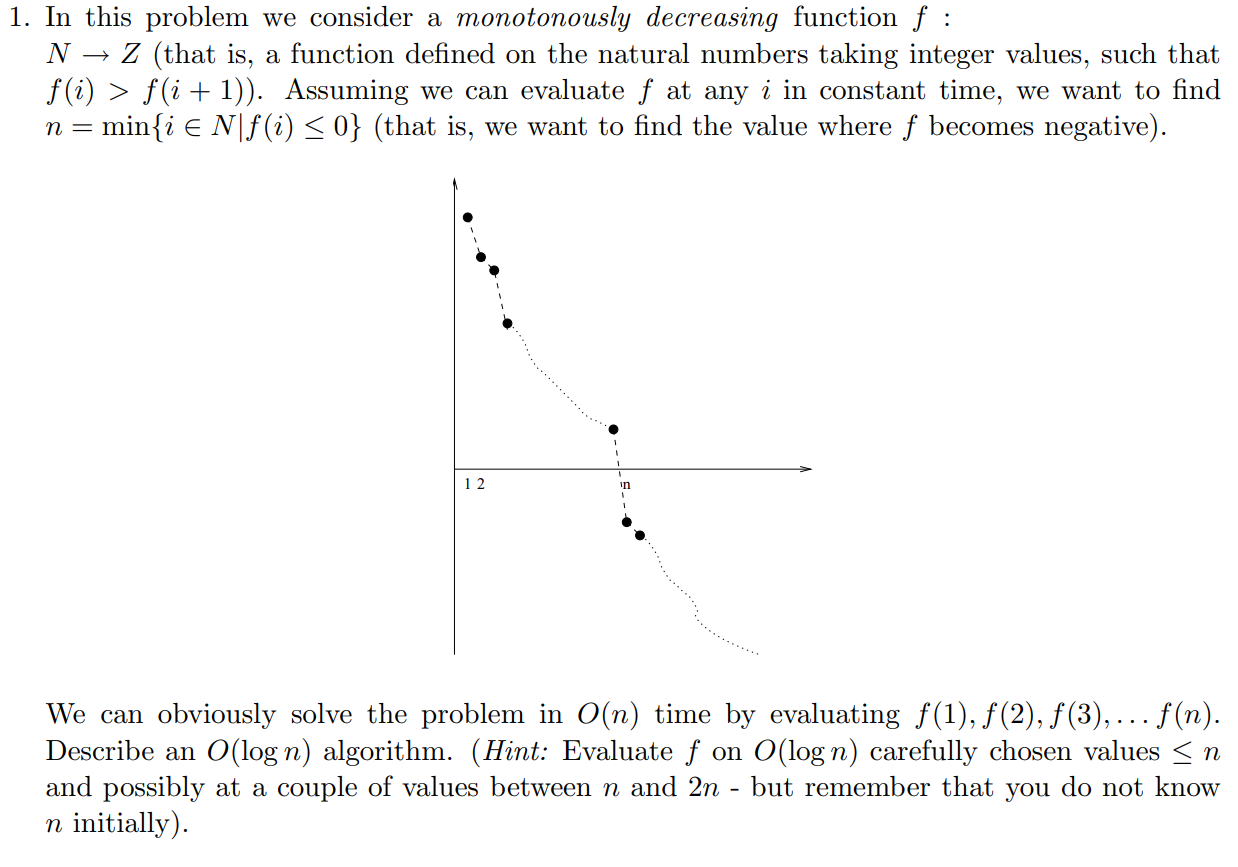
\includegraphics[scale=0.35]{1.png}
\begin{proof}[Solution]
	We can consider the function $f$ as a sorted array that $i$ is the index and $f(i)$ is the value of it.\\
	We need to divide the problem into 2 cases by separate the $i/2$ index each time. Then we may have two cases:\\
	Case 1: median is smaller 0, try to recursively find among the left part\\
	Case 2: median is larger or equal to 0, then try to recursively find among the right part\\
	Both procedure ends when $l>r$.\\
	\begin{lstlisting}[language={python},numbers=left,numberstyle=\tiny,%frame=shadowbox,  
		rulesepcolor=\color{red!20!green!20!blue!20},  
		keywordstyle=\color{blue!70!black},  
		commentstyle=\color{blue!90!},  
		basicstyle=\ttfamily]  
		
	find_first_negative(l,r,arr){
		if(l>r){
			return l<arr.size? l:-1; //-1 means didn't find
		}
		m=(l+r)/2;
		if(arr[m]>=0){
			return find_first_negative(m+1,r,arr);
		}
		if(arr[m]<0){
			return find_first_negative(l,m-1,arr);
		}
	}
	\end{lstlisting}
	$T(n)=T(n/2)+O(1)$, $\log_ba=\log_21$, applying Master theorem, we can get $T(n)=O(\log n)$.\\
	
	E.g. If we have a array that $a = {10,8,4,3,1,0,-4,-8,-0}$. Then we first determine the median 2 is larger than 0. After that, we know that we need to find between ${0,-4,-8,0}$, which is index $[m+1:arr.size-1]$. Recursively apply this method, we finally find the first negative is at index 7 (starting 0) with value -4.
\end{proof}




\textbf{5. Design an O(n) algorithm to find the kth smallest element in an array.}
\begin{proof}[Solution]
	We using the Quick Sort like algorithm in this method.\\
	First pick $arr[r]$ as pivot, put all numbers that smaller on left, larger on right, which is similar in Quick Sort. Then we just need to get the pivot index to determine its rank in the array. We have 3 cases when we get the pivot index:\\
	Case 1: index $=$ k-1
	
	Then it has alrealy be the kth number in the array. return the number.\\
	Case 2: index $<$ k-1
	
	Recursively find in the right part until we find.\\
	Case 3: index $>$ k-1
	
	Recursivly find in the left part.
	\begin{lstlisting}[language={python},numbers=left,numberstyle=\tiny,%frame=shadowbox,  
		rulesepcolor=\color{red!20!green!20!blue!20},  
		keywordstyle=\color{blue!70!black},  
		commentstyle=\color{blue!90!},  
		basicstyle=\ttfamily]  
		
	find_kth(arr, l, r, k){
		int i = l, j = r;
		while (i < j)
		{
			i = l, j = r;
			while (i < j && nums[j] >= nums[l])
			--j;
			while (i < j && nums[i] <= nums[l])
			++i;
			swap(nums[i], nums[j]);
		}
		if(i == k-1){
			return a[i];
		}else if(i > k-1){
			return find_kth(arr, l, i-1, k);
		}else{
			return find_kth(arr, i+1, r, k);
		}
	}
	\end{lstlisting}
	Hence, $T(n) = T(n/2) + O(n)$, $\log_ba=\log_21$, applying Master theorem, we get $T(n)=O(n)$.\\
	
	E.g. If we get an array = ${2,8,6,0,9,3,7}$ and want to find the 6th number. Then we pick 7 as the pivot, then after the partition, array $= {2,3,6,0,\quad 7,\quad  9,8}$, which takes $O(n)$ time since we need to compare each value in the array during partitioning process. Then we can find 7 is on the $4th < 6-1$, then we know that we need to find in the right part. After several recursion, we get the final 6th value 8.
\end{proof}
\textbf{8.}\\
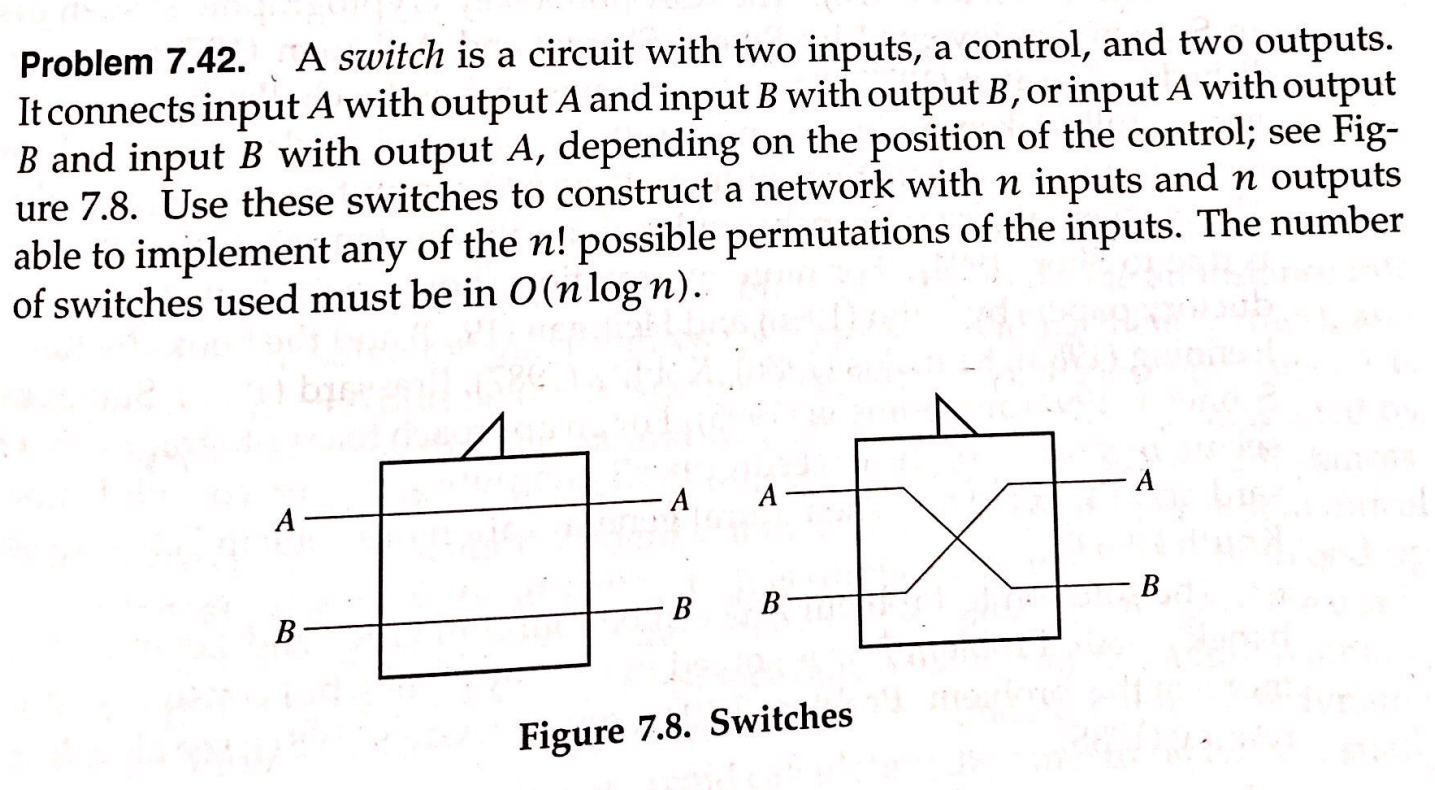
\includegraphics[scale=0.35]{8.png}
\begin{proof}[Solution]
	Divide: divide inputs to 2 groups\\
	Solve subproblem: find all combination of these two groups\\
	Conquer: use $n/2$ case to combine the permutation.\\
	Two base case:
	
	n=2, need 1 switch.
	
	n=1, do not need switch.\\
	Let's take an example of situation $n=4$:\\
	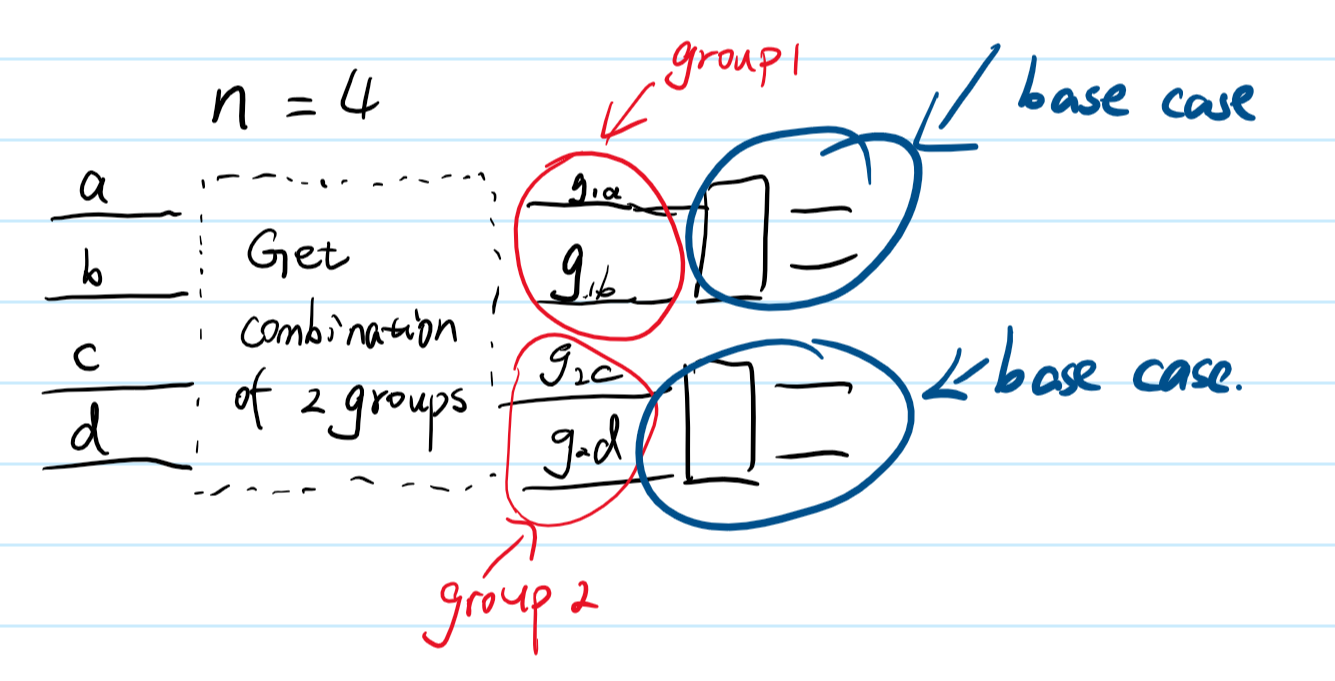
\includegraphics[scale=0.35]{82.png}\\
	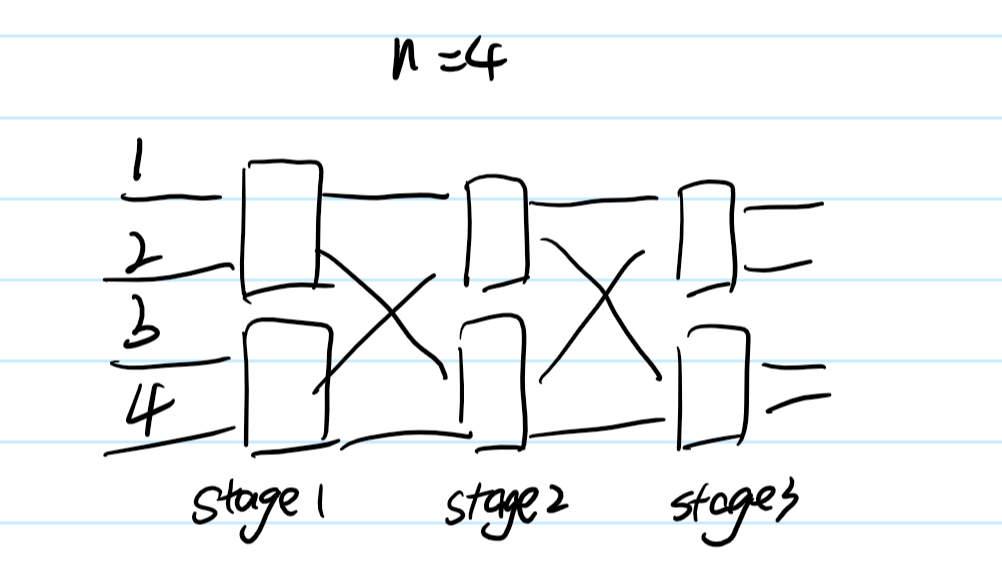
\includegraphics[scale=0.35]{81.png}\\
	Both stage 1 and stage 2 are supposed to get the combination of two group. Therefore, after the stage 2, we can get two group, such as:\[\{1,2\},\{3,4\}\],\[\{1,3\},\{2,4\}\],\[\{2,3\},\{1,4\}\],\[\{1,4\},\{2,3\}\],\[\{2,4\},\{1,3\}\],\[\{3,4\},\{1,2\}\].(remove repetition) Hence, after we find all combination of the two group, our subproblem change to find all permutation of 2 inputs, which is our base case.\\
	For n=8, we used the similar strategy:\\
	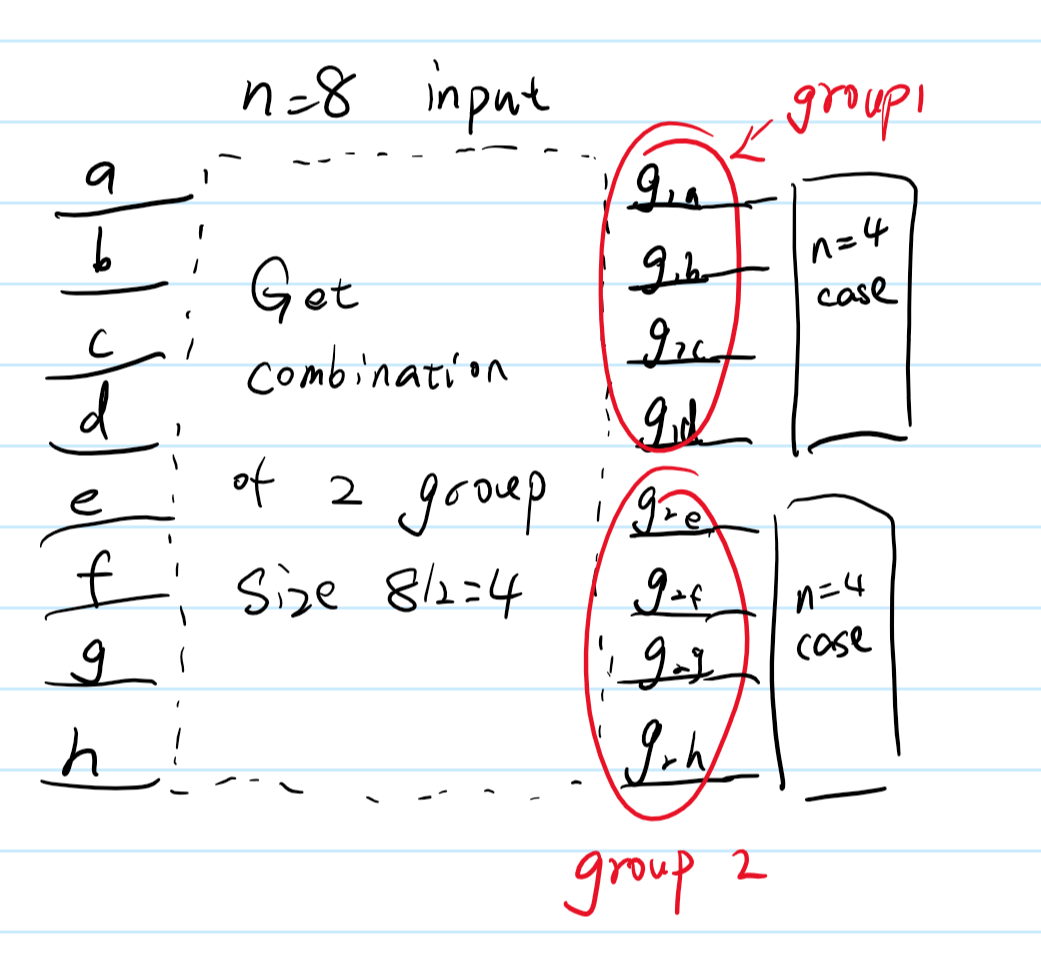
\includegraphics[scale=0.35]{83.png}\\
	For general case, it's like this:\\
	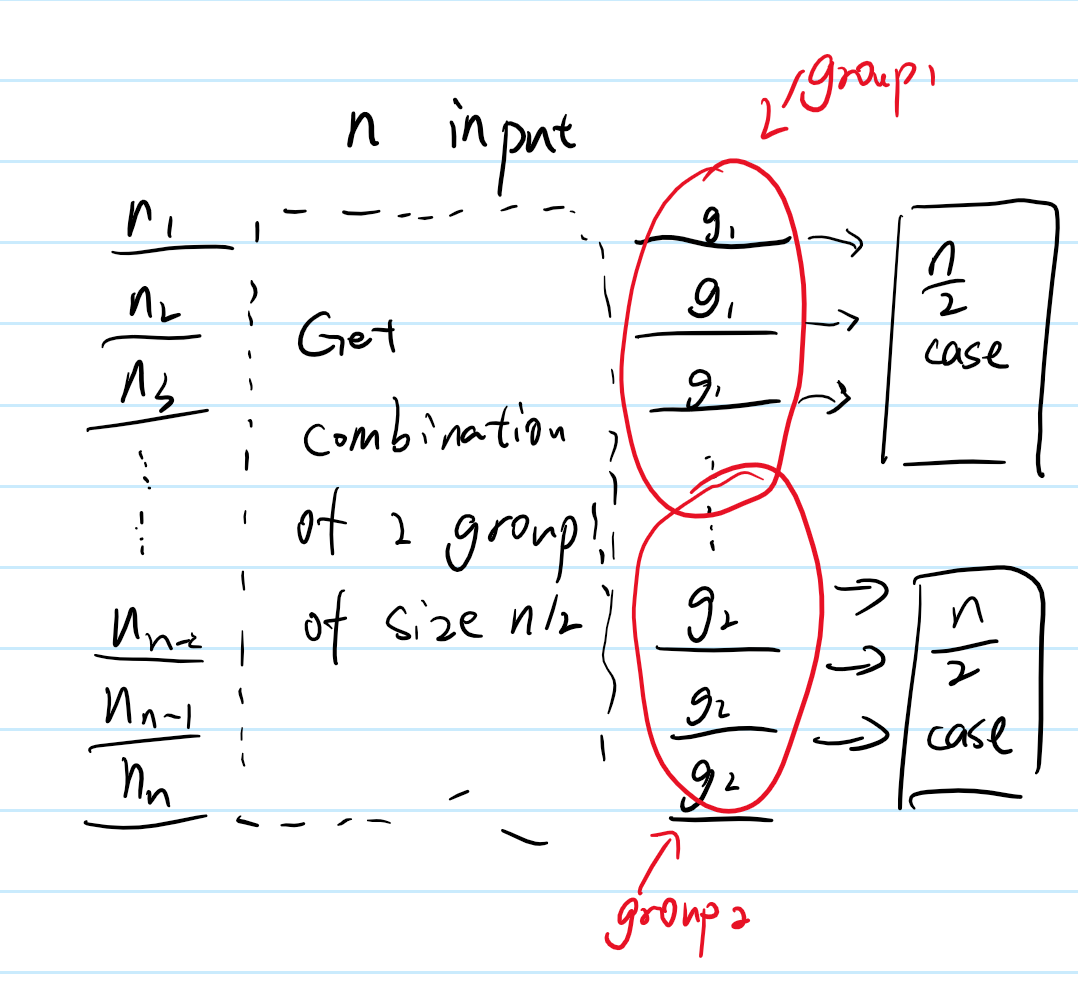
\includegraphics[scale=0.35]{84.png}\\
	Now we need to discuss about how many switches we need in process of computing combination of two groups. For the stage 1, we need to switch element in group1 with corresponding one in group2, which needs $n/2$ switches. Then for stage 2, we need to keep the result before switching them, unless we will lose the original combination. This stage also needs $n/2$ switches. Thus we need $n$ switches to get all combination of 2 group. Assume $S(n)$ is the number of switches we need. We divide the problem by 2 in each loop and generate 2 subproblems, so $S(n)=2S(n/2)+n$, by applying the Master Theorem, we can get $S(n)=O(n\log n)$
	
	
\end{proof}

\bigskip


\begin{thebibliography}{pdf}

\end{thebibliography}
\end{document}
